\documentclass[pdftex,12pt,a4paper]{article}

\usepackage[pdftex]{graphicx}
\usepackage{graphicx}
\usepackage{picture}
\usepackage{graphics}
\usepackage{amsmath} % for argmax
\usepackage{bm} % used for bolding the equation

\newcommand{\HRule}{\rule{\linewidth}{0.5mm}}
\DeclareMathOperator*{\argmin}{argmin}

\begin{document}

\begin{titlepage}

\begin{center}


% Upper part of the page

\includegraphics[width=0.15\textwidth]{./uml_logo}\\[5cm]    

\textsc{\LARGE Computer Graphics I}\\[1.5cm]

\textsc{\Large Literature Reivew III}\\[0.5cm]


% Title
\HRule \\[0.4cm]
{ \huge \bfseries Local deep feature learning framework for 3D shape}\\[0.4cm]

\HRule \\[1.5cm]

% Author and supervisor
\begin{minipage}{0.4\textwidth}
\begin{flushleft} \large
\emph{Author:}\\
Chang \textsc{Liu}
\end{flushleft}
\end{minipage}
\begin{minipage}{0.4\textwidth}
\begin{flushright} \large
\emph{Teacher:} \\
Dr.~Haim \textsc{Levkowitz}
\end{flushright}
\end{minipage}

\vfill

% Bottom of the page
{\large \today}

\end{center}

\end{titlepage}

\section{Abstract}
Object recognition, human pose estimation are applications which are frequently solved through a decomposition into a collection of parts. Detection and recognition require modelling the appearance of the different object parts, and it also requires to model the spatial layout. These representation has already been shown successfully in body part estimation from depth images.

In today's top research in this area, deep learning has gradually shown its full potential, by integrating spatial layout into parts classification without costly pairwise terms during testing, the paper shows that the method classifies pixels independently with a very high precision using convolution neural network.

\section{Overview}
The selected papers are ''\textbf{Human body part estimation from depth images via spatially-constrained deep learning}'' and ''\textbf{Local deep feature learning framework for 3D shape}''. The reason that I choose these two papers are that I find that deep features are a very popular topic in graphic research, how to represent the image or 3D shape well is closely in relation to the feature selection. By choosing different models and feature representation, we could get very different performance and accuracy. In these two papers, the authors both give a very detailed description about the feature selection and how it works in mathematical theory, and I find that by understanding their model, I could get a basic knowledge behind them, and may apply them to my research in the future.

\subsection{}



\section{ANNOR}



\section{Contribution}


\section{Comparable paper}

\section{Descriptor}

\subsection{EHD}


\begin{center} % add this to make the figure shows in the middle of the pages
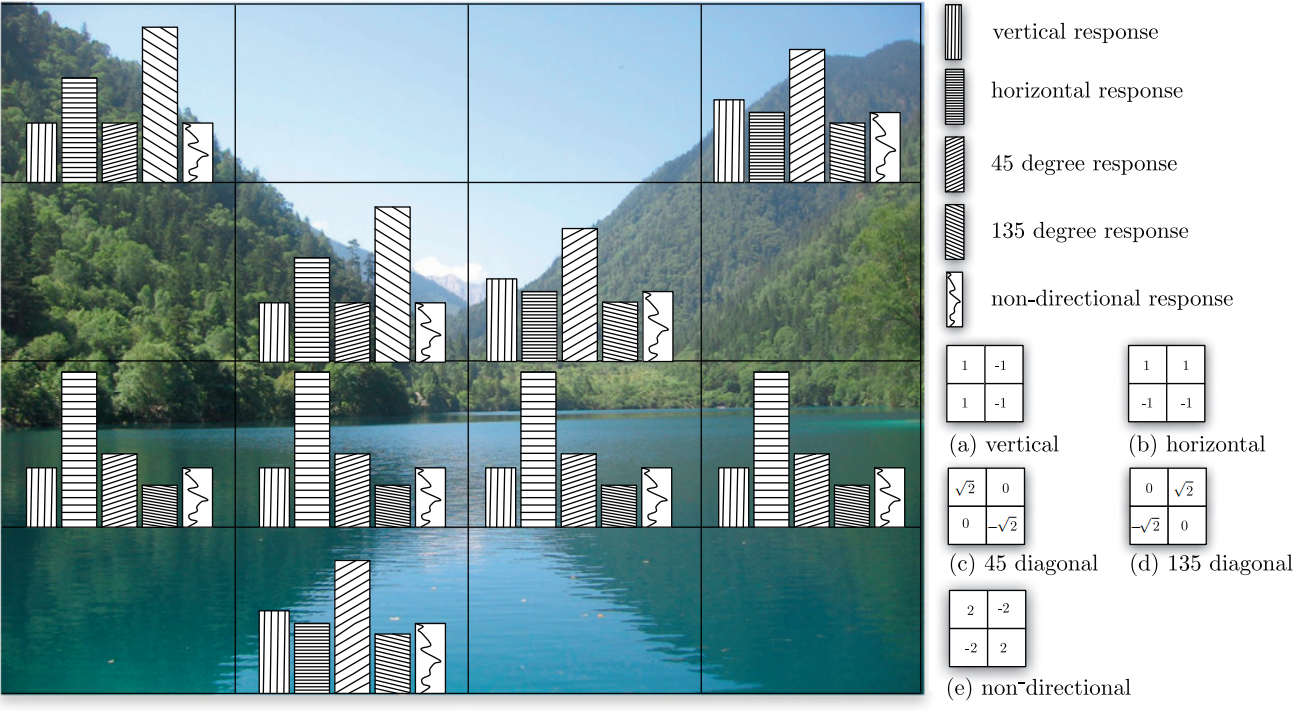
\includegraphics[width=4.00in,height=2.00in]{let-rev2_1.png}
%\caption{EHD descriptor for distinguishing the image}
\end{center}




\section{Tensor descriptor}



\section{Summary}


\section{Reference}
1) Bu, Shuhui, Pengcheng Han, Zhenbao Liu, Junwei Han, and Hongwei Lin. "Local deep feature learning framework for 3D shape." Computers  and Graphics 46 (2015): 117-129.

\noindent 2) Jiu, Mingyuan, Christian Wolf, Graham Taylor, and Atilla Baskurt. "Human body part estimation from depth images via spatially-constrained deep learning." Pattern Recognition Letters 50 (2014): 122-129.

\end{document}